\documentclass[professionalfonts]{beamer}
\newif\ifanswers
%\answerstrue % comment out to hide answers
\answersfalse
\usepackage[familydefault,light]{Chivo} 
\usepackage[T1]{fontenc}
\usenavigationsymbolstemplate{}
\usepackage[]{hyperref}
\usepackage{tikz,pgf,pgfarrows,pgfnodes,pgfbaseimage}
\graphicspath{{./Pics/}}
\usetikzlibrary{shapes}
\usepackage{setspace}
\newcommand{\evi}[1]{{\colorbox{yellow!50}{{#1}}}}
\newcommand{\exe}[1]{{\color{black!50}{{#1}}}}
\newcommand{\kw}[1]{{\colorbox{black!30}{\color{white}{#1}}}}
\tikzstyle{nd}=[circle,draw=black,thick,minimum size=.8cm,inner sep=1pt]
\setbeamercovered{transparent}
\usetheme{Singapore}
\tikzstyle{nodo}=[ellipse,draw=black!60,fill=black!10,line width=.7pt,minimum width=.7cm,minimum height=.4cm]
\usecolortheme[named=gray]{structure}
\setbeamercolor{block title}{bg=black!20,fg=black}
\setbeamercolor{block body}{bg=black!10,fg=black}

\ifanswers
\title{Algoritmi Numerici (Parte I)}
\subtitle{[Lezione 4 bis] Formato Float\\(numeri denormalizzati e precisione)}
\else
\title{Numerics (Part I)}
\subtitle{[Lecture 4 bis] Floating-Point\\(denormal numbers and precision)}
\fi
\date{}
\author{Alessandro Antonucci\\{\tt alessandro.antonucci@supsi.ch}}
%%%%%%%%%%%%%%%%%%%%%%%%%%%%
%%%%%%%%%%%%%%%%%%%%%%%%%%%%

%%%%%%%%%%%%%%%%%%%%%%%%%%%%
\begin{document}
\maketitle
\frame{\frametitle{\ifanswers Il formato {\tt float} (32 bit) \else Format {\tt float} (32 bits) \fi}
\setstretch{1.4}
\begin{center}
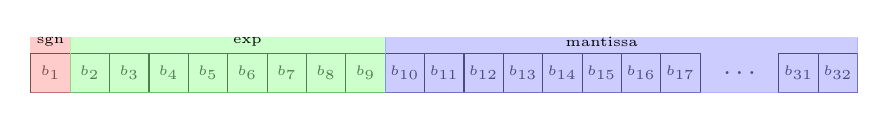
\begin{tikzpicture}[scale=.5]
\draw (-3,0) +(-.5,-.5) rectangle ++(.5,.5); \draw (-2,0) +(-.5,-.5) rectangle ++(.5,.5); \draw (-1,0) +(-.5,-.5) rectangle ++(.5,.5); \draw (0,0) +(-.5,-.5) rectangle ++(.5,.5); \draw (1,0) +(-.5,-.5) rectangle ++(.5,.5); \draw (2,0) +(-.5,-.5) rectangle ++(.5,.5); \draw (3,0) +(-.5,-.5) rectangle ++(.5,.5); \draw (4,0) +(-.5,-.5) rectangle ++(.5,.5); \draw (5,0) +(-.5,-.5) rectangle ++(.5,.5); \draw (6,0) +(-.5,-.5) rectangle ++(.5,.5); \draw (7,0) +(-.5,-.5) rectangle ++(.5,.5); \draw (8,0) +(-.5,-.5) rectangle ++(.5,.5); \draw (9,0) +(-.5,-.5) rectangle ++(.5,.5); \draw (10,0) +(-.5,-.5) rectangle ++(.5,.5); \draw (11,0) +(-.5,-.5) rectangle ++(.5,.5); \draw (12,0) +(-.5,-.5) rectangle ++(.5,.5); \draw (13,0) +(-.5,-.5) rectangle ++(.5,.5); \draw (16,0) +(-.5,-.5) rectangle ++(.5,.5); \draw (17,0) +(-.5,-.5) rectangle ++(.5,.5);
\draw (-3,0) node{\tiny $b_1$}; \draw (-2,0) node{\tiny $b_2$}; \draw (-1,0) node{\tiny $b_3$}; \draw (0,0) node{\tiny $b_4$}; \draw (1,0) node{\tiny $b_5$}; \draw (2,0) node{\tiny $b_6$}; \draw (3,0) node{\tiny $b_7$}; \draw (4,0) node{\tiny $b_8$}; \draw (5,0) node{\tiny $b_9$}; \draw (6,0) node{\tiny $b_{10}$}; \draw (7,0) node{\tiny $b_{11}$}; \draw (8,0) node{\tiny $b_{12}$}; \draw (9,0) node{\tiny $b_{13}$}; \draw (10,0) node{\tiny $b_{14}$}; \draw (11,0) node{\tiny $b_{15}$}; \draw (12,0) node{\tiny $b_{16}$}; \draw (13,0) node{\tiny $b_{17}$}; \draw (16,0) node{\tiny $b_{31}$}; \draw (17,0) node{\tiny $b_{32}$}; \draw (14.5,0) node{$\ldots$}; 
\filldraw[color=red!40,semitransparent] (-3.5,-.50) rectangle (-2.5,.9);
\filldraw[color=green!40,semitransparent] (-2.5,-.50) rectangle (5.5,.9);
\filldraw[color=blue!40,semitransparent] (5.5,-.50) rectangle (17.5,.9);
\draw (-3,+.8) node{\tiny sgn};
\draw (2,+.8) node{\tiny exp};
\draw (11,+.8) node{\tiny mantissa};
\end{tikzpicture}
\end{center}
\begin{itemize}
\item IF $b_1=0$ THEN sgn = +1 \vskip 1mm ELSE sgn = -1
\item exp = {\tt horner}$(b_2 b_3 \ldots b_9)$ - 127
\item mantissa = $1.[b_{10} b_{11} \ldots b_{32}]_2$
\item number = sgn $\cdot$ mantissa $\cdot$ $2^\mathrm{exp}$
\item RETURN number
\end{itemize}}
\frame{\frametitle{\ifanswers Il formato {\tt double} \else Format {\tt double} \fi(64 bit)}
\setstretch{1.4}
\begin{center}
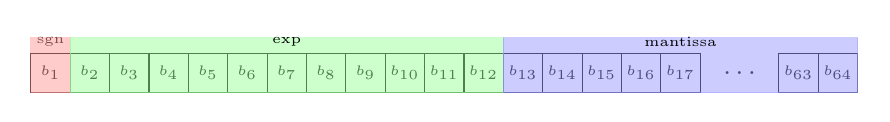
\begin{tikzpicture}[scale=.5]
\draw (-3,0) +(-.5,-.5) rectangle ++(.5,.5); \draw (-2,0) +(-.5,-.5) rectangle ++(.5,.5); \draw (-1,0) +(-.5,-.5) rectangle ++(.5,.5); \draw (0,0) +(-.5,-.5) rectangle ++(.5,.5); \draw (1,0) +(-.5,-.5) rectangle ++(.5,.5); \draw (2,0) +(-.5,-.5) rectangle ++(.5,.5); \draw (3,0) +(-.5,-.5) rectangle ++(.5,.5); \draw (4,0) +(-.5,-.5) rectangle ++(.5,.5); \draw (5,0) +(-.5,-.5) rectangle ++(.5,.5); \draw (6,0) +(-.5,-.5) rectangle ++(.5,.5); \draw (7,0) +(-.5,-.5) rectangle ++(.5,.5); \draw (8,0) +(-.5,-.5) rectangle ++(.5,.5); \draw (9,0) +(-.5,-.5) rectangle ++(.5,.5); \draw (10,0) +(-.5,-.5) rectangle ++(.5,.5); \draw (11,0) +(-.5,-.5) rectangle ++(.5,.5); \draw (12,0) +(-.5,-.5) rectangle ++(.5,.5); \draw (13,0) +(-.5,-.5) rectangle ++(.5,.5); \draw (16,0) +(-.5,-.5) rectangle ++(.5,.5); \draw (17,0) +(-.5,-.5) rectangle ++(.5,.5);
\draw (-3,0) node{\tiny $b_1$}; \draw (-2,0) node{\tiny $b_2$}; \draw (-1,0) node{\tiny $b_3$}; \draw (0,0) node{\tiny $b_4$}; \draw (1,0) node{\tiny $b_5$}; \draw (2,0) node{\tiny $b_6$}; \draw (3,0) node{\tiny $b_7$}; \draw (4,0) node{\tiny $b_8$}; \draw (5,0) node{\tiny $b_9$}; \draw (6,0) node{\tiny $b_{10}$}; \draw (7,0) node{\tiny $b_{11}$}; \draw (8,0) node{\tiny $b_{12}$}; \draw (9,0) node{\tiny $b_{13}$}; \draw (10,0) node{\tiny $b_{14}$}; \draw (11,0) node{\tiny $b_{15}$}; \draw (12,0) node{\tiny $b_{16}$}; \draw (13,0) node{\tiny $b_{17}$}; \draw (16,0) node{\tiny $b_{63}$}; \draw (17,0) node{\tiny $b_{64}$}; \draw (14.5,0) node{$\ldots$}; 
\draw (-3,+.8) node{\tiny sgn};
\filldraw[color=red!40,semitransparent] (-3.5,-.50) rectangle (-2.5,.9);
\filldraw[color=green!40,semitransparent] (-2.5,-.50) rectangle (8.5,.9);
\filldraw[color=blue!40,semitransparent] (8.5,-.50) rectangle (17.5,.9);
\draw (3,+.8) node{\tiny exp};
\draw (13,+.8) node{\tiny mantissa};
\end{tikzpicture}
\end{center}
\begin{itemize}
\item 1/11/52 bits sgn/exp/mantissa \exe{float 1/8/23)}
\item exp - 1023 ($=2^{11-1}-1$ \exe{float $127=2^{8-1}-1$})
\end{itemize}
\begin{itemize}
\item IF $b_1=0$ THEN sgn = +1 ELSE sgn = -1
\item exp = {\tt horner}$(b_2 b_3 \ldots b_{12})$ - 1023
\item mantissa = $1.[b_{13} b_{14} \ldots b_{64}]_2$
\end{itemize}}

\frame{\frametitle{5-bits float-like}
\begin{columns}
\begin{column}[T]{0.1\textwidth}
\end{column}
\begin{column}[T]{0.5\textwidth}
\tiny
1/2/2 bits sgn/exp/mantissa,\\exp - $2^{2-1}-1=1$
\small
\vskip 2mm
$0|00|00 \to + 1.00_2 \cdot 2^{-1}= 0.5$\\
$0|00|01 \to + 1.01_2 \cdot 2^{-1}=0.625$\\
$0|00|10 \to + 1.10_2 \cdot 2^{-1}=0.75$\\
$0|00|11 \to + 1.11_2 \cdot 2^{-1}=0.875$\\
$0|01|00 \to + 1.00_2 \cdot 2^0=1$\\
$0|01|01 \to + 1.01_2 \cdot 2^0=1.25$\\
$0|01|10 \to + 1.10_2 \cdot 2^0=1.5$\\
$0|01|11 \to + 1.11_2 \cdot 2^0=1.75$\\
$0|10|00 \to + 1.00_2 \cdot 2^1=2$\\
$0|10|01 \to + 1.01_2 \cdot 2^1=2.5$\\
$0|10|10 \to + 1.10_2 \cdot 2^1=3$\\
$0|10|11 \to + 1.11_2 \cdot 2^1=3.5$\\
$0|11|00 \to + 1.00_2 \cdot 2^2=4$\\
$0|11|01 \to + 1.01_2 \cdot 2^2=5$\\
$0|11|10 \to + 1.10_2 \cdot 2^2=6$\\
$0|11|11 \to + 1.11_2 \cdot 2^2=7$
\end{column}
\begin{column}[T]{0.4\textwidth}
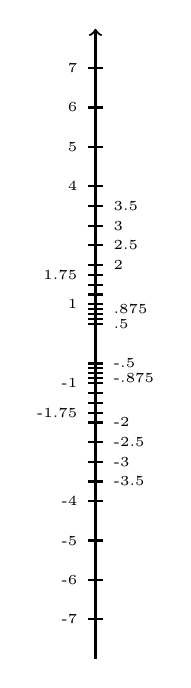
\begin{tikzpicture}[scale=.5]
\draw[->,thick] (0,-8) -- (0,8);
\draw[left,thick] (.2,7) -- (-.2,7) node[] {\tiny 7};
\draw[left,thick] (.2,6) -- (-.2,6) node[] {\tiny 6};
\draw[left,thick] (.2,5) -- (-.2,5) node[] {\tiny 5};
\draw[left,thick] (.2,4) -- (-.2,4) node[] {\tiny 4};
\draw[right,thick] (-.2,3.5) -- (.2,3.5) node[] {\tiny 3.5};
\draw[right,thick] (-.2,3) -- (.2,3) node[] {\tiny 3};
\draw[right,thick] (-.2,2.5) -- (.2,2.5) node[] {\tiny 2.5};
\draw[right,thick] (-.2,2) -- (.2,2) node[] {\tiny 2};
\draw[left,thick] (.2,1.75) -- (-.2,1.75) node[] {\tiny 1.75};
\draw[left,thick] (.2,1.5) -- (-.2,1.5) node[] {};
\draw[left,thick] (.2,1.25) -- (-.2,1.25) node[] {};
\draw[left,thick] (.2,1) -- (-.2,1) node[] {\tiny 1};
\draw[right,thick] (-.2,.875) -- (.2,.875) node[] {\tiny .875};
\draw[right,thick] (-.2,.75) -- (.2,.75) node[] {};
\draw[right,thick] (-.2,.625) -- (.2,.625) node[] {};
\draw[right,thick] (-.2,.5) -- (.2,.5) node[] {\tiny .5};
\draw[right,thick] (-.2,-.875) -- (.2,-.875) node[] {\tiny -.875};
\draw[right,thick] (-.2,-.75) -- (.2,-.75) node[] {};
\draw[right,thick] (-.2,-.625) -- (.2,-.625) node[] {};
\draw[right,thick] (-.2,-.5) -- (.2,-.5) node[] {\tiny -.5};
\draw[left,thick] (.2,-1) -- (-.2,-1) node[] {\tiny -1};
\draw[left,thick] (.2,-1.25) -- (-.2,-1.25) node[] {};
\draw[left,thick] (.2,-1.5) -- (-.2,-1.5) node[] {};
\draw[left,thick] (.2,-1.75) -- (-.2,-1.75) node[] {\tiny -1.75};
\draw[right,thick] (-.2,-2) -- (.2,-2) node[] {\tiny -2};
\draw[right,thick] (-.2,-2.5) -- (.2,-2.5) node[] {\tiny -2.5};
\draw[right,thick] (-.2,-3) -- (.2,-3) node[] {\tiny -3};
\draw[right,thick] (-.2,-3.5) -- (.2,-3.5) node[] {\tiny -3.5};
\draw[left,thick] (.2,-4) -- (-.2,-4) node[] {\tiny -4};
\draw[left,thick] (.2,-5) -- (-.2,-5) node[] {\tiny -5};
\draw[left,thick] (.2,-6) -- (-.2,-6) node[] {\tiny -6};
\draw[left,thick] (.2,-7) -- (-.2,-7) node[] {\tiny -7};
\end{tikzpicture}\end{column}\end{columns}}

\frame{\frametitle{\ifanswers I formati float-like \else Float-like Formats \fi}
\begin{block}{\ifanswers Vantaggio \else Pros \fi}
\ifanswers
Numeri macchina vicini fra loro vicino allo zero \\
pi\`u distanti per numeri grandi (in valore assoluto)
\vskip 1mm
Errore di rappresentazione cresce in termini assoluti,\\
costante in termini relativi
\else
Small numbers? Machine numbers are close\\
Increased separation for larger numbers
\vskip 1mm
Absolute error in representation increases with larger numbers, relative remains constant!
\fi
\end{block}
\vskip 2mm
\begin{block}{\ifanswers Svantaggio \else Cons \fi}
\ifanswers
numero macchina pi\`u piccolo in valore assoluto $\neq 0$\\
\else
smallest machine number (absolute value) $\neq 0$\\
\fi
\vskip 1mm
$0|00000000|00\ldots 00 = + 1.0 \cdot 2^{-127} = \frac{1}{2^{127}} \neq 0$\\
$1|00000000|00\ldots 00 = - 1.0 \cdot 2^{-127} = -\frac{1}{2^{127}}$
\end{block}}

\frame{\frametitle{\ifanswers Mantissa denormalizzata \else Denormalized Mantissa \fi}
\begin{block}{
\ifanswers Eccezione al formato {\tt float} per avere $0$ numero macchina
\else
{\tt float} format exceptions to make $0$ a machine number
\fi
}
\begin{itemize}
\item IF $(b_2,\ldots,b_9)=(000000000)$ THEN
\item mantissa = $0.[b_{10} b_{11} \ldots b_{32}]_2$ (denormalized)
\item exp = -126 (no 0-127=-127!)
\end{itemize}
\end{block}
\begin{centering}
$0|00000000|0\ldots 0=+0.0$
\quad $1|00000000|0\ldots 0=-0.0$
\end{centering}
\vskip 3mm
\begin{itemize}
\item \ifanswers Zero macchina ($0_m$) pi\`u piccolo numero macchina \else Machine zero ($0_m$) smallest machine number \fi
(non-zero)
\item \ifanswers Mantissa denormalizzata produce $0_m$ 
molto pi\`u piccolo \else Denormalized mantissa makes $0_m$ much smaller \fi
\item \ifanswers Stessa cosa per {\tt double}, con -1022
\else Same story with {\tt double}, -1022 \fi
\item \ifanswers $(b_2,\ldots,b_9)=(111111111)$ eccezione per \else $(b_2,\ldots,b_9)=(111111111)$ exception for  $\pm \infty$ e $NaN$ \fi
\end{itemize}}


\frame{\frametitle{\ifanswers Stima dell'errore di rappresentazione\else Estimating the representation error\fi}
\setstretch{1.4}
\begin{itemize} 
\item \ifanswers Rappresentazione \else Representation \fi float $x_m = \pm 1.[b_{10},b_{11},\ldots,b_{32}]_2 \cdot 2^p$
\item \ifanswers ``Vero'' numero \else ``True'' number \fi $x =  \pm 1.[b_{10} b_{11} \ldots b_{32} b_{33} b_{34} \ldots]_2 \cdot 2^p$
\item \ifanswers Se il formato float facesse troncamento:
\else A float doing truncation:
\fi
 $\epsilon_a = |x - x_m| = \left| 0.[00 \ldots 0b_{33} b_{34} \ldots]_2 \right| \cdot 2^p$
\item $\epsilon_a = |x - x_m| = |0.[b_{33}b_{34}\ldots]_2| 2^{p-23}<2^{p-23}$
\item $\epsilon_r = | \frac{x_m-x}{x} | = \frac{\epsilon_a}{|x|} < \frac{2^{p-23}}{|x|} < 2^{-23}$
\ifanswers
perch\'e \else because \fi $x \geq 1.0000 \cdot 2^{p}$
\item 
\ifanswers
Il formato float arrotonda, stime errori sono la met\`a!
\else
Float is rounding, errors are the half! \fi
\end{itemize}
}

\frame{\frametitle{\ifanswers Stima dell'errore di rappresentazione (con't)\else Estimating the representation error (con't)\fi}
\setstretch{1.4}
\begin{itemize} 
\item \ifanswers Se $p$ \`e l'esponente del numero da rappresentare (in base 2 e con mantissa normalizzata)
\else
Let $p$ denote the exponent of the number to represent
(base 2, mantissa normalized)
\fi
\item \ifanswers Se $s$ \`e il numero di bit a disposizione per la mantissa
\else
Le $s$ denote the number of bits to store the mantissa
\fi
\end{itemize}
\begin{columns}
\begin{column}[T]{0.5\textwidth}
\begin{block}{\small \ifanswers con TRONCAMENTO \else with TRUNCATION \fi}
\begin{center}
$\epsilon_a < 2^{p-s}$
\vskip 1mm
$\epsilon_r < 2^{-s}$
\end{center}
\end{block}
\end{column}
\begin{column}[T]{0.5\textwidth}
\begin{block}{\small \ifanswers con ARROTONDAMENTO \else with ROUNDING \fi}
\begin{center}
$\epsilon_a < 2^{p-s-1}$
\vskip 1mm
$\epsilon_r < 2^{-s-1}$
\end{center}
\end{block}
\end{column}
\end{columns}
\vskip 1mm 
{\tt float} $\epsilon_r < 2^{-24} \simeq 6 \cdot 10^{-8}$, 7/8 \ifanswers cifre corrette \else right digits \fi(base 10)\\
{\tt double} $\epsilon_r < 2^{-53} \simeq 1.1 \cdot 10^{-16}$, 15/16 \ifanswers cifre corrette \else right digits \fi}

\end{document}

\frame{\frametitle{Esercizio}
\Large
\begin{center}
Analizza come si modifica il formato a 5 bit
\vskip 1mm
introdotto precedentemente 
\vskip 1mm
quando si considera anche l'eccezione
\vskip 1mm
per la mantissa denormalizzata 
\end{center}}

\frame{\frametitle{Soluzione}
\begin{columns}
\begin{column}[T]{0.1\textwidth}
\end{column}
\begin{column}[T]{0.5\textwidth}
\tiny
1/2/2 bit per segno/espo/mantissa, espo - $2^{2-1}-1=1$
\small
\vskip 2mm
$0|00|00 \to + 0.00_2 \cdot 2^{0}= 0.0$\\
$0|00|01 \to + 0.01_2 \cdot 2^{0}=0.25$\\
$0|00|10 \to + 0.10_2 \cdot 2^{0}=0.5$\\
$0|00|11 \to + 0.11_2 \cdot 2^{0}=0.75$\\
$0|01|00 \to + 1.00_2 \cdot 2^0=1$\\
$0|01|01 \to + 1.01_2 \cdot 2^0=1.25$\\
$0|01|10 \to + 1.10_2 \cdot 2^0=1.5$\\
$0|01|11 \to + 1.11_2 \cdot 2^0=1.75$\\
$0|10|00 \to + 1.00_2 \cdot 2^1=2$\\
$0|10|01 \to + 1.01_2 \cdot 2^1=2.5$\\
$0|10|10 \to + 1.10_2 \cdot 2^1=3$\\
$0|10|11 \to + 1.11_2 \cdot 2^1=3.5$\\
$0|11|00 \to + 1.00_2 \cdot 2^2=4$\\
$0|11|01 \to + 1.01_2 \cdot 2^2=5$\\
$0|11|10 \to + 1.10_2 \cdot 2^2=6$\\
$0|11|11 \to + 1.11_2 \cdot 2^2=7$
\end{column}
\begin{column}[T]{0.4\textwidth}
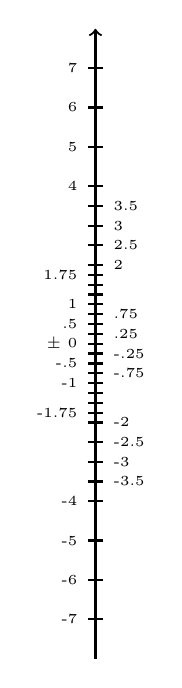
\begin{tikzpicture}[scale=.5]
\draw[->,thick] (0,-8) -- (0,8);
\draw[left,thick] (.2,7) -- (-.2,7) node[] {\tiny 7};
\draw[left,thick] (.2,6) -- (-.2,6) node[] {\tiny 6};
\draw[left,thick] (.2,5) -- (-.2,5) node[] {\tiny 5};
\draw[left,thick] (.2,4) -- (-.2,4) node[] {\tiny 4};
\draw[right,thick] (-.2,3.5) -- (.2,3.5) node[] {\tiny 3.5};
\draw[right,thick] (-.2,3) -- (.2,3) node[] {\tiny 3};
\draw[right,thick] (-.2,2.5) -- (.2,2.5) node[] {\tiny 2.5};
\draw[right,thick] (-.2,2) -- (.2,2) node[] {\tiny 2};
\draw[left,thick] (.2,1.75) -- (-.2,1.75) node[] {\tiny 1.75};
\draw[left,thick] (.2,1.5) -- (-.2,1.5) node[] {};
\draw[left,thick] (.2,1.25) -- (-.2,1.25) node[] {};
\draw[left,thick] (.2,1) -- (-.2,1) node[] {\tiny 1};
\draw[right,thick] (-.2,.75) -- (.2,.75) node[] {\tiny .75};
\draw[left,thick] (.2,.5) -- (-.2,.5) node[] {\tiny .5};
\draw[right,thick] (-.2,.25) -- (.2,.25) node[] {\tiny .25};
\draw[left,thick] (.2,0) -- (-.2,.0) node[] {\tiny $\pm$ 0};
\draw[right,thick] (-.2,-.75) -- (.2,-.75) node[] {\tiny -.75};
\draw[left,thick] (.2,-.5) -- (-.2,-.5) node[] {\tiny -.5};
\draw[right,thick] (-.2,-.25) -- (.2,-.25) node[] {\tiny -.25};
\draw[left,thick] (.2,-1) -- (-.2,-1) node[] {\tiny -1};
\draw[left,thick] (.2,-1.25) -- (-.2,-1.25) node[] {};
\draw[left,thick] (.2,-1.5) -- (-.2,-1.5) node[] {};
\draw[left,thick] (.2,-1.75) -- (-.2,-1.75) node[] {\tiny -1.75};
\draw[right,thick] (-.2,-2) -- (.2,-2) node[] {\tiny -2};
\draw[right,thick] (-.2,-2.5) -- (.2,-2.5) node[] {\tiny -2.5};
\draw[right,thick] (-.2,-3) -- (.2,-3) node[] {\tiny -3};
\draw[right,thick] (-.2,-3.5) -- (.2,-3.5) node[] {\tiny -3.5};
\draw[left,thick] (.2,-4) -- (-.2,-4) node[] {\tiny -4};
\draw[left,thick] (.2,-5) -- (-.2,-5) node[] {\tiny -5};
\draw[left,thick] (.2,-6) -- (-.2,-6) node[] {\tiny -6};
\draw[left,thick] (.2,-7) -- (-.2,-7) node[] {\tiny -7};
\end{tikzpicture}\end{column}\end{columns}}

\frame{\frametitle{Esercizio 1}
\setstretch{1.4}
\begin{itemize}
\item Scrivere la sequenza che codifica il numero x=50.02 secondo le regole del formato {\tt float}
\item Se il numero non \`e un numero macchina calcolare l'errore assoluto verificando che sia inferiore al valore di stima pessimistica
\item Ripetere la stessa analisi per l'errore relativo
\end{itemize}}

\frame{\frametitle{Esercizio 1 (i)}
Converto separatamente il 50 ed il .02 in base 2
\begin{columns}
\begin{column}[T]{0.1\textwidth}
\end{column}
\begin{column}[T]{0.4\textwidth}
\vskip 5mm
50 mod 2 = 0\\
25 mod 2 = 1\\
12 mod 2 = 0\\
6 mod 2 = 0\\
3 mod 2 = 1\\
1 mod 2 = 1
\vskip 2mm
$50 = 110010_2$
\end{column}
\begin{column}[T]{0.4\textwidth}
\vskip 5mm
\tiny
int(.02 x 2) = 0\\
int(.04. x 2) = 0\\
int(.08. x 2) = 0\\
int(.16 x 2) = 0\\
int(.32 x 2) = 0\\
int(.64 x 2) = 1\\
int(.28 x 2) = 0\\
int(.56 x 2) = 1\\
int(.12 x 2) = 0\\
int(.24 x 2) = 0\\
int(.48 x 2) = 0\\
int(.96 x 2) = 1\\
int(.92 x 2) = 1\\
int(.84 x 2) = 1\\
int(.68 x 2) = 1\\
int(.36 x 2) = 0\\
int(.72 x 2) = 1\\
int(.44 x 2) = 0\\
int(.88 x 2) = 1\\
int(.76 x 2) = 1\\
int(.52 x 2) = 1\\
int(.04 x 2) =
\vskip 2mm
$0.02 = 0.0\overline{00001010001111010111}_2$
\end{column}
\end{columns}}

\frame{\frametitle{Esercizio 1 (ii)}
50.02 = $110010.0\overline{00001010001111010111}_2$
\vskip 2mm
In notazione scientifica $+1.100100\overline{00001010001111010111} \cdot 2^{5}$
\vskip 2mm
Esponente 5 come qualcosa meno 127, il valore \`e 132
\vskip 2mm
132 come un numero naturale in base 2 ad 8 bit
{\small
\vskip 2mm
132 mod 2 = 0\\
66 mod 2 = 0\\
33 mod 2 = 1\\
16 mod 2 = 0\\
8 mod 2 = 0\\
4 mod 2 = 0\\
2 mod 2 = 0\\
1 mod 2 = 1}
\vskip 2mm
132 = 1000|0100
}


\frame{\frametitle{Esercizio 1 (iii)}
in grigio i bit della mantissa dopo il 23-esimo
\vskip 2mm
$+1.100100\overline{00001010001111010\color{black!30}{111}} \cdot 2^{\mathrm{Horner}(1000|0100)-127}$
\vskip 2mm
Con troncamento, approssimo per difetto:
\vskip 2mm
$+1.10010000001010001111010 \cdot 2^{\mathrm{Horner}(1000|0100)-127}$
\vskip 2mm
Ma il formato float fa arrotondamento,\vskip 1mm
approssimo per eccesso (primo bit fuori uno):
\vskip 2mm
$x = +1.10010000001010001111011 \cdot 2^{\mathrm{Horner}(1000|0100)-127}$
\vskip 2mm
ovvero 
\vskip 2mm
0|10000100|10010000001010001111011 $\to$ 4248147B}
\frame{\frametitle{Esercizio 1 (iv)}
Per valutare l'errore assoluto leggo il numero macchina:
\vskip 2mm
$0|10000100|10010000001010001111011$
\vskip 2mm
$+1.10010000001010001111011 \cdot 2^5 =$ 
\vskip 2mm
$110010.000001010001111011$
\vskip 2mm
A sx della virgola 50
\vskip 2mm
A dx (in esadecimale) .0000|0101|0001|1110|1100=.051EC
}

\frame{\frametitle{Esercizio 1 (v)}
C/16 + E = 12/16+14 = 14.75\\
14.75/16+1 = 1.921785\\
1.921785/16+5 = 5.1201171875\\
5.1201171875/16+0 = 0.32000732421875\\
0.32000732421875/16 = 0.020000457763671875\\
\vskip 3mm
Il numero macchina e' quindi 50.020000457763671875
\vskip 2mm
 (leggermente piu' grande di 50.02 in seguito all'approssimazione per eccesso)
\vskip 2mm
L'errore "esatto" \`e quindi
$0.000000457763671875 = 4.57763671875 10^{-7}$
\vskip 1mm
minore del valore di stima pessimistico (errore assoluto per arrotondamento con 23 bit di mantissa)\\
\vskip 1mm
$2^{p-s-1}=2^{5-23-1}=2^{-19}=\frac{1}{524288} \simeq 1.9073\cdot 10^{-6}$}

\frame{\frametitle{Esercizio 1 (vi)}
Per l'errore relativo
\vskip 2mm
Valore ``esatto''\\
$\epsilon_r = 0.000000457763671875/50.02 \simeq 9.151612792383045 \cdot 10^{-9}$
\vskip 2mm
Valore pessimistico $2^{-24} \simeq 
5.960464477539063\cdot 10^{-8}$
\vskip 2mm
La formula \`e rispettata
}
\frame{\frametitle{Esercizio 2}
Scrivere il numero $-0.5 \cdot 2^{-128}$ secondo le regole del formato float.
\vskip 2mm
$-0.5 \cdot 2^{-128} = -.1_2 2^{-128} = - 1.0 2^{-129}$
\vskip 2mm
L'esponente -129 non si pu\`o esprimere come $k-127$
\vskip 2mm
Devo lavorare con mantissa denormalizzata
$-1.0 \cdot 2^{-3} \cdot 2^{-126} =-0.001 \cdot 2^{-126}$
\vskip 2mm
sequenza bit
$1|00000000|0010 \ldots 0 \to 80010000$
}

\frame{\frametitle{Esercizio 3}
Scrivere il numero $2^{-128}+2^{-150}$ secondo le regole del formato float.
\vskip 2mm
Raccolgo $2^{-128}$:
\vskip 1mm
$2^{-128} (1+2^{-22}) = + 1.\overbrace{00\ldots00}^{21 zeri}1 \cdot 2^{-128}$
\vskip 1mm
Esponente $-128$: troppo piccolo per mantissa normalizzata!
\vskip 2mm
Uso mantissa denormalizzata, esponente $=-126$, virgola mantissa si sposta di due posizioni a sx per compensare:
\begin{center}
$+0.01\overbrace{00\ldots00}^{21 zeri}1 \cdot 2^{-126}$
\end{center}
24 bit dopo virgola, approssimo a: $+0.\overbrace{0100\ldots01}^{23 bits} \cdot 2^{-126}$
Sequenza 32 bits: {\footnotesize 0|00000000|01000000000000000000001}}
\end{document}
